\documentclass[11pt,space]{ctexart} 
\usepackage[ans]{GEEexam_Quant}

\usepackage{enumitem} % 引入enumitem包
\setlist[itemize]{label=\textbullet}
\usepackage{tabularx}

\usepackage{tikz}
\renewcommand{\oval}{
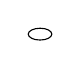
\begin{tikzpicture}
  \draw (0,0) ellipse (.15cm and .075cm);
\end{tikzpicture}
}

\newcommand{\options}[5]{
\begin{center}
\begin{tabularx}{\linewidth}{>{\raggedleft\arraybackslash}p{0.45\linewidth} p{0.5\linewidth}}
    \oval & {#1} \\
    \oval & {#2} \\
    \oval & {#3} \\
    \oval & {#4} \\
    \oval & {#5}
\end{tabularx}
\end{center}
}

\newcommand{\quantities}[2]{
\begin{center}
    \begin{tabularx}{\linewidth}{*{2}{>{\centering\arraybackslash}X}}
    \textbf{\underline{Quantity A}} & \textbf{\underline{Quantity B}}\\
    {#1} & {#2}
    \end{tabularx}
\end{center}
    
\begin{center}
\begin{tabularx}{\linewidth}{>{\raggedleft\arraybackslash}p{0.2\linewidth} p{0.8\linewidth}}
    \oval & Quantity A is greater. \\
    \oval & Quantity B is greater. \\
    \oval & The two quantities are equal. \\
    \oval & The relationship cannot be determined from the information given.
\end{tabularx}
\end{center}
}
\renewcommand{\note}[1]{{\heiti\textbf{注\hspace{1em}}}#1.}

\newcommand{\field}{
\begin{center}
\begin{tikzpicture}
  \draw (0,0) rectangle (3,.6);
\end{tikzpicture}
\end{center}
}

\begin{document}

\begin{enumerate}

\item $y = 105n$ ($n$ is a positive integer). $y$ is both the square of an integer, and a multiple of $30$. What is the least possible value of $n$?
\field
\note{y 是 $105$ 和 $30$ 的公倍数，而 $105 = 5 \times 3 \times 7$，$30 = 2 \times 3 \times 5$，所以 $105$ 和 $30$ 的最小公倍数为 $2 \times 3 \times 5 \times 7 = 210$。那么，$y$ 只需要是 $210$ 的倍数即可。但是 $y$ 还是一个整数的平方，因为 $210$ 的质因数都是一次方，所以至少让它们都升到平方才能是完全平方数，即 $210^2 = 44100$ 是最小的既是完全平方数又是 $210$ 的倍数的数。此时 $y = 105n$，那么解得 $n = 420$}

\item $n$ is an integer greater than $1,000$.
\quantities{The number of prime numbers greater than $n$ and less than $n+15$}{6}
\note{从 \( n+1 \) 到 \( n+14 \) 当中，有7个奇数和7个偶数。7个偶数肯定不是质数。3的倍数在每3个连续整数中一定会有一个，因此，在14个连续整数当中，起码有4个是3的倍数，其中2个是3的偶数倍，另外2个是3的奇数倍。因此，在7个奇数中，至少还可以再排除2个是3的奇数倍的数，它们也不是质数。因此，质数的数量最多是 \( 7 - 2 = 5 \) 个，\( QA \) 的最大值小于6，因此 \( QA < QB \)}

\item In a probability experiment, events \( R, S, \) and \( T \) are such that \( P(S) = P(T) = x \), \( P(R) = kx \), and \( P(R \text{ or } S) < P(S \text{ or } T) \), where \( k \) and \( x \) are positive numbers. Events \( R \) and \( S \) are mutually exclusive, and events \( S \) and \( T \) are independent.
\quantities{$k$}{$1-x$}
\note{$R$和$S$是互斥事件，$P(R \text{ or } S) = P(R)+P(S) = kx+x$. $S$和$T$独立，$P(S\text{ and }T) = P(S)P(T) = x^2$.因此，$P(S \text{ or }T) = P(S)+P(T)-P(S \text{ and } T = x+x-x^2$}

\item What is the remainder when $8^{43}$ is divided by $7$?
\field
\note{$8^{43} = (7+1)^{43} = \{7\text{的倍数}\}+1^{43}$，因此余数就是$1$}

\item The repeating decimal \( 1.\overline{ab} \), where \( a \) and \( b \) are different digits, is equivalent to the fraction \( \frac{n}{d} \), where \( n \) and \( d \) are positive integers whose greatest common factor is 1. What is the greatest possible value of \( n + d \) ?
\options{296}{297}{298}{299}{301}
\note{回忆一下初中是怎么证明$0.\overline{3} = 1$的。
\begin{equation*}
    \begin{aligned}
        & 1.\overline{ab} = \frac{n}{d}\\
        \implies & 100\cdot 1.\overline{ab} = 1ab+0.\overline{ab} = 100\frac{n}{d}\\
        \implies & 1ab-1 = 99\frac{n}{d}\\
    \iff & \frac{n}{d} = \frac{1ab-1}{99}
    \end{aligned}
\end{equation*}
又因为$a$和$b$是不同的数字，因此$1ab$的最大值为$198$，这时$\frac{n}{d} = \frac{198}{99}$。又因为$n$和$d$互质，所以$n = 198$，$d = 99$，$n+d = 296$
}

\item How many integers between $360$ and $630$ are there such that they have odd number of divisors?
\options{3}{4}{5}{6}{7}
\note{将一个数质因数分解，可以表达为$a_1^{b_1}a_2^{b_2}\cdots$，那么它的因数的个数为$(b_1+1)(b_2+1)\cdots$，因为每一个质因数$a_i$的幂次都可以在$0,1,\cdots,b_i$做选择。要让质因数个数为奇数，那么只有可能是每一个$(b_i+1)$都是奇数，那么每一个$b_i$则都是偶数。记$b_i = 2k_i$，则这个数也可以表示为$a_1^{b_1}a_2^{b_2}\cdots = a_1^{2k_1}a_2^{2k_2}\cdots = \left(a_1^{k_1}a_2^{k_2}\cdots\right)^2$，得出这个数必然是完全平方数。$19^2 = 361$，$25^2 = 625$，从$19$到$25$共有7个完全平方数，也就是7个有奇数个因数的数。作为补充，如果一个数只有3个因数，那么这个数必然是某质数的平方}

\item If \( a \), \( b \), and \( c \) are positive integers such that \( \dfrac{a}{c} = 0.075 \), and \( \dfrac{b}{c} = 0.09 \), what is the least possible value of \( c \)?
\field
\note{
\begin{equation*}
    \begin{aligned}
        & \dfrac{a}{c} = 0.075 \iff a = \frac{3}{40}c\\
        & \dfrac{b}{c} = 0.09 \iff b = \frac{9}{100}c
    \end{aligned}
\end{equation*}
为了让$a$和$b$都是整数，$c$必须同时是40和100的倍数。40和100的最小公倍数是200
}

\item $n$ is an integer greater than $3$.
\quantities{The fraction of the integers greater than $1$ and less than $n$ that are prime numbers}{$\frac{1}{2}$}
\note{当视野放到足够远时，所有除了2之外的偶数必然不是质数，还有一些奇数可能会是$3, 5, 7$等的倍数，所以质数的比例一定小于$\frac12$。最特殊的情况在于2是偶数也是质数，以及10以下的质数很多。当$n \le 10$时，从$2$到$(n-1)$中质数的比例都会大于$\frac12$}

\item $k$ is a positive integer.
\quantities{The number of prime numbers from $k$ to $k+10$}{The number of prime numbers from $k+10$ to $k+20$}
\note{大的趋势来说，数字越大后质数越少，不可能是相等关系。也不可能是严格的大小关系，不然总可以推出$k$足够大时，$k$到$k+10$有11个或者0个质数，这是不可能的。答案只有可能是二者的大小不定，这也符合直觉}

\item $p$ and $r$ are different prime numbers greater than $3$.
\quantities{The number of positive factors of $pr^2$}{The number of positive factors of $(p+3)(r+3)$}
\note{因为$p$和$r$都是质数，并且$p\ne r$，故$pr^2$的因数有$(1+1)(2+1) = 6$个。又因为$p$和$r$都是大于3的质数，所以$p$和$r$都是奇数，$(p+3)$和$(r+3)$都是偶数，故$(p+3)(r+3)$必定有2和$4\ (=2\times 2)$作为因子，本身也有$1,(p+3),(r+3),(p+3)(r+3)$作为因子。再考虑到2和4作为因子时，还有$\dfrac{(p+3)(r+3)}{2}$和$\dfrac{(p+3)(r+3)}{4}$作为因子，因此$(p+3)(r+3)$的因子数比$pr^2$的更多}

\item How many integers from 1 to 2,000, inclusive, are both the square of an integer and the cube of an integer?
\options{3}{4}{12}{22}{44}
\note{
根据题意，该整数$m$一定能写成$m = a^3 = b^2$，其中$a$是一个完全平方数，$b$是一个完全立方数；因此$m$也一定可以写成$m = (n^2)^3 = (n^3)^2 = n^6$，所以满足题意的$m$一定会是某个数字的六次方。$1^6 = 6$，$2^6 = 64$，$3^6 = 729$，$4^6 = 4096>2000$，因此一共有3个这样的数.

穷举法就不多说了。这道题也可以用一种简单的找规律破解。如若把一个整数$m$写成整数$a$的三次方，$m = a\times a \times a$，为了让$m$同时能够是另一个整数的平方，中间的$a$一定能够拆成两个完全相同的整数（记为$b$）相乘，这样有$m = a\times b \times b \times a = (ab)\times (ba) = (ab)^2$。$12^3<2000$，$13^3>2000$，在1到12中，一共只有$1,4,9$三个整数是完全平方数，因此满足题目要求的数也只有3个
}

\item List $A$ consists of 25 positive integers $a_1,a_2,a_3,\cdots,a_{25}$ that are ordered from least to greatest. The median and the mode of the integers in $A$ are both equal to 10. List $B$ consists of 25 positive integers \( b_1, b_2, b_3, \ldots, b_{25} \) that are ordered from least to greatest. The median and the mode of the integers in \( B \) are both equal to 15. List \( C \) consists of the 25 sums \( a_i + b_i \), for all integers \( i \) such that \( 1 \leq i \leq 25 \). The mode of the integers in \( C \) is \( m \).
\quantities{The median of the integers in $C$}{$m$}
\note{$QA$和$QB$要相等是容易的。若考虑反例，巧妙地考虑$A$和$B$中众数的位置可能会“错开”，比如
\begin{itemize}
    \item List $A$: 10 10 10 15 25
    \item List $B$: 10 10 15 15 15
\end{itemize}
则List $C$为 20 20 25 30 40，构成反例
}

\item $ABCD$ is a quadrilateral. 
\quantities{The perimeter of $ABCD$}{The sum of the lengths of diagonals $AC$ and $BD$}
\note{
由三角形两边之和大于第三边，有
\begin{equation*}
    \begin{aligned}
        & \begin{cases}
            A B + B C > A C \\
            A D + D C > A C \\
            A B + A D > B D \\
            C B + C D > B D 
        \end{cases}\\
        \implies & 2(A B + B C + C D + D A) > 2(A C + B D)\\
        \implies & A B + B C + C D + D A > A C + B D
    \end{aligned}
\end{equation*}
或者，用一种更暴力的“两边之和大于第三边”：假设对角线$AC$和$BD$交于点$O$，则有
\begin{equation*}
    \begin{aligned}
        & \begin{cases}
            AB>OA\\
            BC>OB\\
            CD>OC\\
            AD>OD
        \end{cases}\\
        \implies & A B + B C + C D + D A > OA+OB+OC+OD=AC+BD
    \end{aligned}
\end{equation*}
补充一点，没有一个四边形的性质阐述了周长和对角线长度和的关系
}

\item Let $S$ be the set of integers from 1 to 10. How many subsets of $S$ contain at least one even integer and at least one odd integer?
\options{25}{31}{62}{252}{961}
\note{这道题讲究方法和技巧的结合：
\begin{itemize}
    \item 大小为10的集合的所有子集个数为$2^{10} = 1024$，料想到被排除的子集数量绝对小于一半（大小大于等于6的子集必满足要求，小于6的也没有全被排除），直接排除法选出961.
    \item 正着算不好算，则反着算。考虑子集全是奇数或者全是偶数的情况，这就相当于分别求全集是奇数或者偶数的子集数量：各$2^5 = 32$个。注意这其中空集被计算了两次，所以不满足题目要求的子集数量为$32\times 2-1 = 63$，满足题目要求的子集数量为$2^{10}-63=961$.
\end{itemize}
补充一点，$\sum_{k = 0}^n\mathrm{C}_{n}^k = 2^n$
}

\item Professor Lopez is teaching three different courses with an average (arithmetic mean) enrollment of 32 students per course. If 5 students are taking two of these courses, 3 other students are taking all three courses, and all of the others are taking only one of the courses, what is the total number of different students enrolled in the three courses?
\field
\note{
可以用最朴素的加法。三门课的学生数直接相加时，选两门课的人被加了2次（多加了1次），选三门课的人被加了3次（多加了2次）。排除掉多加的部分即为学生数，即$96-5\cdot 1-3\cdot 2 = 85$.

也可以先排除出去所有多加的情况，剩下的都是只选一门课的学生，即$96-2\cdot 5-3\cdot 3 = 77$，然后再补加回那些学生，$77+5+3 = 85$.

注意这里容斥原理不能直接用，因为三个集合两两交集的大小没有直接给出，应该是$5+3\cdot 3 = 14$（因为每两个集合的交集都会包含三个集合的交集一次）。用上容斥原理得出学生数为$96-14+3 = 85$
}

\item During archery practice, Kyle made 50 attempts to hit a target. After each attempt, his success rate was calculated as the number of successful attempts to hit the target as a percent of the number of attempts up to that time. After the 20th attempt, his success rate was 45 percent. After the 40th attempt, his success rate was 55 percent. Which of the following statements must be true?

Indicate all such statements.

\begin{center}
\begin{tabularx}{\linewidth}{>{\raggedleft\arraybackslash}p{0.05\linewidth} p{0.95\linewidth}}
    $\square$ & Kyle's success rate was less than 45 percent at least once during the practice. \\
    $\square$ & Kyle's success rate was between 48 percent and 52 percent at least once during the practice. \\
    $\square$ & Kyle's success rate was greater than 55 percent at least once during the practice.
\end{tabularx}
\end{center}

\note{
这题最好是用排除法，很容易找到AC选项的反例，B从直觉上很可能成立（虽然也需要计算验证），直接选B进入下一题.

关于B选项的验证：从第20次到第40次过程当中，Kyle的射击成功率大致需要动态上升，从20次时的45\%增加到第40次时的55\%。每射中一次，那么分子分母同步+1，射击成功率根据糖水不等式上升，但是上升的幅度是否可以一次性从48\%扩大到52\%，跳过中间值，一次性提升4\%？最大的提升幅度必然在于第21次尝试射中，在这之后Kyle的射击成功率为10/21≈47.6\%，比第20次后的45\%提升2.6\%；而接下来，随着分母增加，提升的幅度只会越来越小，所以不可能一次性提升4\%，即不可能突然从48\%，直接一次性跳跃上升到52\%，所以B选项找不到反例，一定会存在至少1次尝试后射击成功率位于48\%和52\%之间，B选项一定成立
}

\newpage
\section*{易错题}

\item A survey conducted by the department of motor vehicles on a sample of 200 car owners revealed that 15\% of the sample had an expired driver's license, 10\% had one or more outstanding parking tickets, and 78\% had neither an expired driver's license nor any outstanding parking tickets. How many car owners in the sample had both an expired driver's license and one or more outstanding parking tickets?
\options{3}{6}{8}{9}{10}
\note{留心总人数！这类集合和比例的问题一定要注意提供的信息是绝对人数还是百分比，也要注意所有关于比例的信息的“分母”或者“整体”都是什么}

\item How many integers between 37 and 621 are squares of even integers?
\options{9}{10}{15}{17}{18}
\note{
两个易错点：
\begin{itemize}
    \item 题目问的是在37和621之间能成为偶数平方的整数个数，并不是问有多少偶数的平方能落在37和621之间。
    \item 计算出最小偶数为8，最大偶数为24，计算总偶数个数时不要直接$24-8+1=17$，这样是无形中把8和24之间的全部数字都算上了（包括奇数），要注意只能算上偶数！
\end{itemize}
另外，如果真的问到开平方，不要忘了负数
}

\item $x^2+y^2 = 52$. Both $x$ and $y$ are integers and $x>y$.
\quantities{$x$}{$4$}
\note{考虑$x$和$y$可能的正负}

\item $n$ is an integer.
\quantities{$\left(\frac23\right)^n\left(32\right)^{-n}$}{1}
\note{考虑$n$有可能是负数，不要想当然地只考虑正整数}\

\item $c$ and $d$ are positive integers.
\quantities{$\dfrac{c}{d}$}{$\dfrac{c+3}{d+3}$}
\note{
糖水不等式有使用条件！$c,d,x>0$，当$c<d$，即$\frac{c}{d}<1$时，才有
\begin{equation*}
    \frac{c}{d}<\frac{c+x}{d+x}
\end{equation*}
这边没有给出$c$和$d$的大小关系，故不能直接使用糖水不等式。我的建议是，GRE的题目都不复杂，最好不要轻易用二级结论，因为很多二级结论都有使用条件，忽视了这些条件可能会导致误判，从零开始推导反而能做对
}

\item The probability that each toss of a certain coin will result in heads is \( 0.5 \). If the probability that \( n \) tosses of the coin will each result in heads is greater than \( 0.0002 \), what is the greatest possible value of \( n \)?
\field
\note{考试中的计算器不能计算$\log$，这里要转化为可比较的关系，然后逐渐尝试。
\begin{equation*}
    \begin{aligned}
        & \left(\frac12\right)^n>0.0002 = \frac{1}{5000}\\
        \iff & 2^n<5000\\
        \implies & n\le 12 \ (2^{12} = 4096)
    \end{aligned}
\end{equation*}
另外，考试的计算器也不能开根号和直接算平方，都需要合理转化
}

\newpage
\section*{留心字面理解}

\item 
\quantities{The number of tenths equal to 1.4}{The number of hundredths equal to 1.3}
\note{tenth意为“十分之一”，即0.1；hundreth意为“百分之一”，即0.01}

\item A simple sailboat often has two sails, the mainsail and the headsail, as shown in the figure above. A recreational sailor is building a simple sailboat and is designing each sail to be in the shape of a right triangle. The mainsail will have a height of 12 feet and a hypotenuse of length 15 feet. The headsail will have a height of 15 feet and a hypotenuse of length 16.25 feet. Based on the design, the area of the mainsail will be how much greater than the area of the headsail?

Give your answer to the nearest square foot.

\field
\note{由"nearest"，答案的要求是“四舍五入保留到最近的整数”}

\item Three lamps had the same original price, but they were sold at different selling prices: A, B, and C.
\begin{itemize}
    \item Selling price A was obtained by applying a 75\% discount to the original price.
    \item Selling price B was obtained by applying a 50\% discount to the original price and then applying a 25\% discount to the discounted price.
    \item Selling price C was obtained by applying a 60\% discount to the original price and then applying a 15\% discount to the discounted price.
\end{itemize}
Which of the following shows A, B, and C listed in order from least to greatest?
\options{A, B, C}{A, C, B}{B, C, A}{C, A, B}{C, B, A}
\note{"apply a $x\%$ discount"的含义是打折后售价为原价的$(100-x)\%$}

\item A gardener plans to cover a rectangular plot of land with pine bark mulch to a depth of 4 inches. The plot measures 8 feet by 12 feet, and the gardener will buy mulch packed in bags. If each bag contains 3.5 cubic feet of mulch and costs \$6, what is the cost of the least number of bags that the gardener will need to cover the plot? (Note: 1 foot=12 inches.)
\begin{center}
    \blank{}dollars
\end{center}
\field
\note{应用题注意向上或向下取整}

\item Last year and this year, there were both men and women in a certain choir. This year there are x fewer men and x fewer women in the choir than there were last year, where x>0, and there are fewer men than women in the choir.
\quantities{The percent decrease from last year to this year in the number of men in the choir}{The percent decrease from last year to this year in the number of women in the choir}
\note{不要理解错题意，这边说的是合唱团里男性/女性的数量从去年到今年的下降的百分比，而不是说男性/女性占合唱团总人数百分比从去年到今年的下降}

\end{enumerate}



\end{document}